\documentclass[a4paper, 12pt]{article}
\usepackage{geometry}
\usepackage[russian]{babel}
\usepackage[T2A]{fontenc}
\usepackage{chngcntr}
\usepackage{graphicx}
\usepackage{verbatim}

\begin{document}


\begin{titlepage}

\begin{center}
{\textsc{\textbf{Правительство Российской Федерации}}}\\
\vspace{0.5cm}
\hrule
\vspace{0.5cm}
{\textsc{Федеральное государственное автономное образовательное учреждение\\высшего образования <<Национальный исследовательский университет\\<<Высшая школа экономики>>}}\\
\vspace{1cm}
Кафедра <<Компьютерная безопасность>>
\end{center}

\vspace{\fill}
% Поменять номер лабы
\begin{center}
{\Large{\textbf{ОТЧЕТ \\ К ЛАБОРАТОРНОЙ РАБОТЕ №10}}} \\
\vspace{1em}
{\textbf{по дисциплине}} \\
\vspace{1em}
{\large{\textbf{<<Языки программирования>>}}}
\end{center}

\vspace{\fill}


\begin{flushright}
  \begin{minipage}[center]{15cm}

    \begin{minipage}[left]{5cm}
      {Работу выполнил\\студент группы СКБ-222}
    \end{minipage}
    \begin{minipage}[center]{5cm}
      \vspace{1.25cm}
      \hrulefill\\[-1cm]
      \begin{center}{подпись, дата}\end{center}
    \end{minipage}
    \begin{minipage}[right]{4cm}
      \vspace{0.4cm}
      \begin{flushright}{А.С. Вагин}\end{flushright}
    \end{minipage}
    \\
    \\
    \\
    \begin{minipage}[left]{5cm}
      {Работу проверил}
    \end{minipage}
    \begin{minipage}[center]{5cm}
      \vspace{1.25cm}
      \hrulefill\\[-1cm]
      \begin{center}{подпись, дата}\end{center}
    \end{minipage}
    \begin{minipage}[right]{4cm}
      \begin{flushright}{С.А. Булгаков}\end{flushright}
    \end{minipage}
  \end{minipage}
\end{flushright}

\vspace{\fill}

\begin{center}
Москва~2022
\end{center}
\end{titlepage}
\setcounter{page}{2}
\setcounter{secnumdepth}{5}
\setcounter{tocdepth}{5}

% Содержание
\tableofcontents
\cleardoublepage

\setcounter{section}{1}
\counterwithout{subsection}{section}
\graphicspath{ {./images/} }

% Постановка задачи
\cleardoublepage
\section*{Постановка задачи}\addcontentsline{toc}{section}{Постановка задачи}
% Сюда
\cleardoublepage



\section*{Основная часть}\addcontentsline{toc}{section}{Основная часть}

\subsection{Описание изменений}
% Что-то про прошлые лабы

\subsection{Описание функций}
\subsubsection{Какая-то функция}
% Про новые функции

\cleardoublepage


\section*{Приложение A}\addcontentsline{toc}{section}{Приложение А}
\renewcommand\thesection{\Alph{section}}
\renewcommand\thesubsection{\thesection.\arabic{subsection}}
\setcounter{subsection}{0}

\subsection{UML-диаграмма \textit{clearStdin}}
% 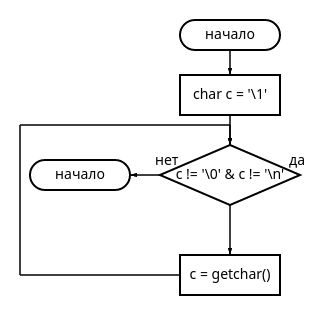
\includegraphics[width=\columnwidth]{clearStdin.png}


\cleardoublepage

\setcounter{subsection}{0}
\section*{Приложение B}\addcontentsline{toc}{section}{Приложение B}
\renewcommand\thesection{\Alph{section}}
\renewcommand\thesubsection{B.\arabic{subsection}}

\subsection{Код программы}

\fontsize{9}{9}\selectfont
% Код сюда
\begin{verbatim}

\end{verbatim}

\end{document}
